\part{运动产生}
\markboth{运动产生}{运动产生}

\chapter{肌肉生物学和力量}\label{chap:chap4}


孤身一人,我们能做的太少。
团结起来,我们能做的却很多。
\begin{flushright}
	————海伦$\cdot$凯勒
\end{flushright}


\begin{figure}[!htb]
	\centering
	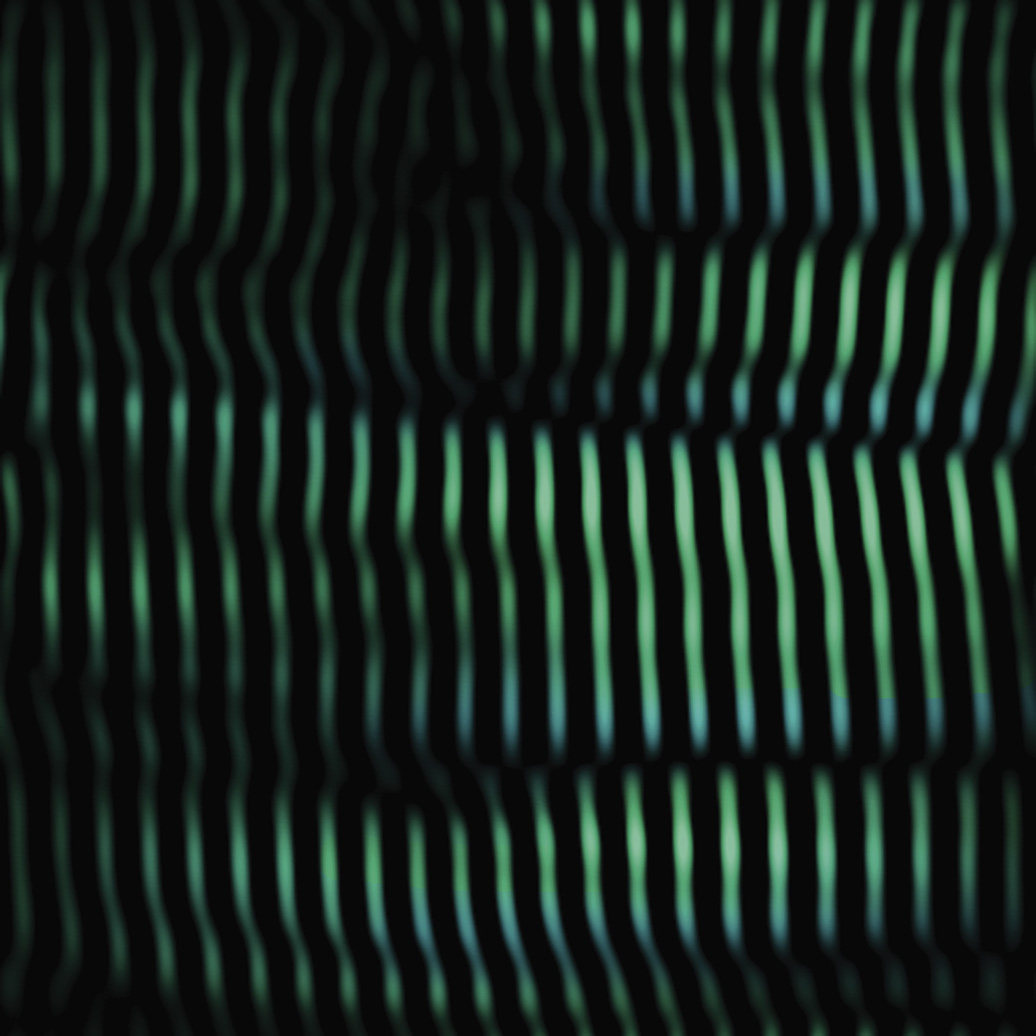
\includegraphics[width=1.0\linewidth]{chap4/4_0}
	% 加星号(*)表示不加编号
	\caption*{ \label{fig:4_0}}
\end{figure}


伦敦皇家学会拥有350年的历史,拥有近200年的传统,每年都会邀请科学家进行公开演讲,并经常进行一些简单的实验。
1952年,其中一项实验成为了热议话题。


两辆固定自行车朝向相反,并通过一条链条连接在一起,当一辆自行车向前踩踏板时,另一辆自行车的踏板就会向后移动(图~\ref{fig:4_1})。


\begin{figure}[!htb]
	\centering
	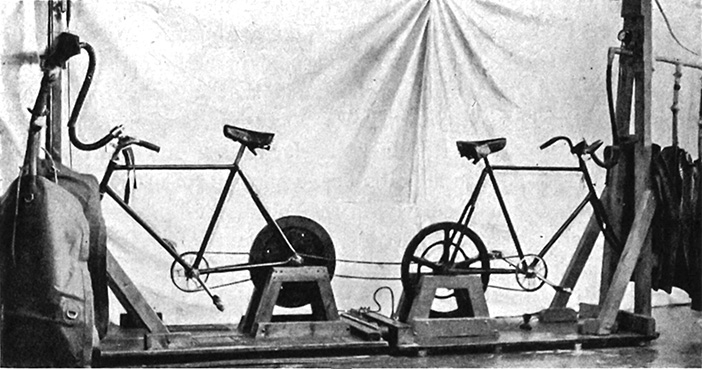
\includegraphics[width=1.0\linewidth]{chap4/4_1}
	\caption{Abbott 等人 (1952) 描述的推拉装置。 \label{fig:4_1}}
\end{figure}


一辆自行车上坐着一位娇小的女子,名叫布伦达$\cdot$比格兰,是肌肉疲劳研究领域的权威专家。
另一辆自行车上坐着一位魁梧的年轻人,名叫默多克$\cdot$里奇,他嫁给了他的自行车“对手”。
演讲者是A$\cdot$V$\cdot$希尔,他因在肌肉产热方面的研究而获得了诺贝尔奖。


里奇听从指令,用尽全力向前蹬,而比格兰则用力蹬着脚蹬,阻止他继续蹬。
想象一下,当观众看到这位娇小的女子轻而易举地阻止了这位身材高大的男人蹬得更快时,他们会有多么惊讶。
很快,他便大汗淋漓,气喘吁吁,而比格兰却几乎毫不费力。
甚至连伦敦市长后来也过来试驾。
“这套设备后来被命名为‘推拉你’,以纪念杜立特医生那只永远不知道自己要往哪个方向跑的双头怪兽,”布伦达$\cdot$比格兰-里奇后来写道。


魔术?小把戏?
并非如此,但它确实表明,肌肉消耗能量和产生力量的方式并非显而易见。
肌肉做正功(例如,在向前蹬踏时充当“马达”)时,它们消耗的能量和产生的热量,比做负功(例如,在向前蹬踏时充当“刹车”)时要多。
一般来说,肌肉产生的力量和消耗的能量,很大程度上取决于它是缩短还是伸长。
希尔实验的经验教训至今仍在日常康复和阻力训练中得到应用。
正如我们将看到的,奇迹发生在分子层面。


本章和下一章将深入探究肌肉内部,探索其结构与功能之间的关系。
肌肉是神奇的生物马达,能够在瞬间悄无声息地产生数千牛顿的力量。
这些力量如此巨大,以至于你小腿的肌肉就能举起一辆小型汽车的尾部。
这些巨大的力量是由数万亿个纳米级分子马达共同作用产生的,这些马达将我们摄入食物中的化学能转化为机械能,使我们能够活动。
这一非凡的功能源于骨骼肌特化的细胞机制和高度组织化的层级结构(图~\ref{fig:4_2})。


\begin{figure}[!htb]
	\centering
	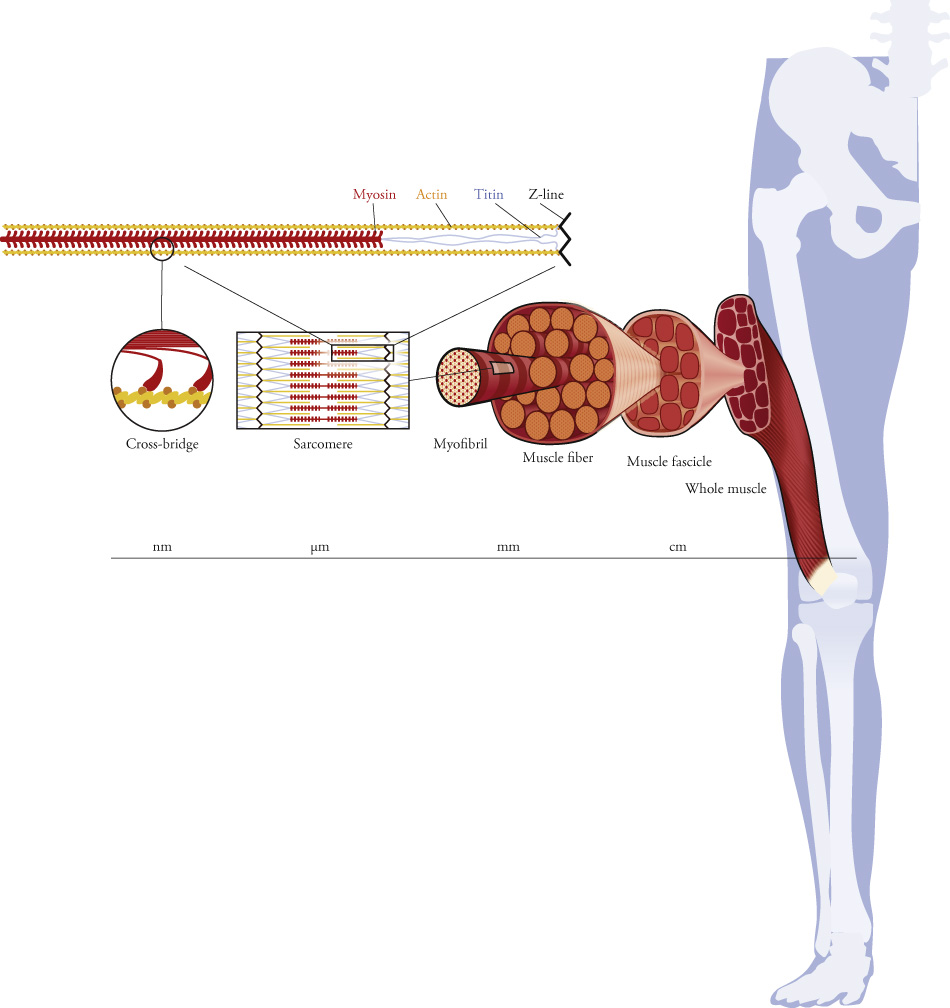
\includegraphics[width=1.0\linewidth]{chap4/4_2}
	\caption{肌肉的多尺度结构。
		骨骼肌具有层次结构,其中有被称为肌球蛋白的纳米级分子马达,每个肌球蛋白仅产生几皮牛顿的力,排列成肌节、肌原纤维、纤维、肌束和整个肌肉,在强力肌肉收缩期间可产生数千牛顿的力。 \label{fig:4_2}}
\end{figure}


接下来两章的组织将大致遵循肌肉的层级结构。
我们将首先在分子层面研究力量的产生过程。
接下来,我们将了解分子马达是如何被包裹在被称为肌节的亚细胞结构中的(活体人体肌节的第一张图像就是在我的手臂上拍摄的,并在本章的开篇图中展示)。
进一步深入,我们将了解单个肌肉细胞如何被神经系统激活,并了解“快肌纤维”和“慢肌纤维”之间的区别。
在第~\ref{chap:chap5}~章中,我们将从宏观层面研究肌肉在体内的排列方式,以及它们如何与肌腱(将肌肉力量传递到骨骼结构)相互作用。


\section{肌肉结构}

从最基本的层面来说,肌肉通过两种细长蛋白质(肌动蛋白和肌球蛋白)的相互作用产生力量。
20 世纪 50 年代初,休$\cdot$赫胥黎通过 X 射线显微镜发现,这些蛋白质平行排列,纤维交织,它们之间的连接被他称为“横桥”。
安德鲁$\cdot$赫胥黎(与休无亲属)同时用不同的方法发现了横桥。
休$\cdot$赫胥黎和安德鲁$\cdot$赫胥黎都怀疑横桥是产生力量的机制,并于 1954 年提出了一个关于这些分子马达如何工作的模型,我们将在下文中解释。
他们的模型一直是解释力量产生的基本范式,尽管随着更多实验数据的收集,该模型变得更加详细。


从尺寸上看,肌纤维排列成束,称为肌束,它们与肌肉纤维一样,长度可达数十厘米。
肌束的横截面积约为 1 毫米。
除了肌纤维外,肌束还包含称为细胞外基质的结缔组织,其中包括胶原蛋白、神经纤维和血管。
在健康的肌肉中,肌纤维紧密排列;
然而,在患病的肌肉中,肌纤维的横截面积可能较小,并被更多的细胞外基质和脂肪隔开。


肌束被更多结缔组织包围,并聚集在一起形成肌肉。
另一层结缔组织鞘被称为筋膜,包裹着肌肉并将其与其他肌肉隔开。
终止于每个肌束末端的肌纤维可以直接附着在骨骼上,但通常它们会连接到肌腱,肌腱随后附着在骨骼上。
肌腱插入肌肉的部分称为腱膜;
肌腱在肌肉外部的部分通常称为游离肌腱。
正如我们将在第~\ref{chap:chap5}~章中看到的,肌腱不仅通过向骨骼传递肌肉力量发挥着重要作用,还在伸展和回缩时储存和释放能量。


\section{横桥循环}

当神经系统激活肌肉时,肌肉会通过数万亿个肌动蛋白和肌球蛋白的协同作用产生力量,这个过程被称为“横桥循环”(图~\ref{fig:4_3})。
这种机制可以粗略地描述为一个分子大小的棘轮。


\begin{figure}[!htb]
	\centering
	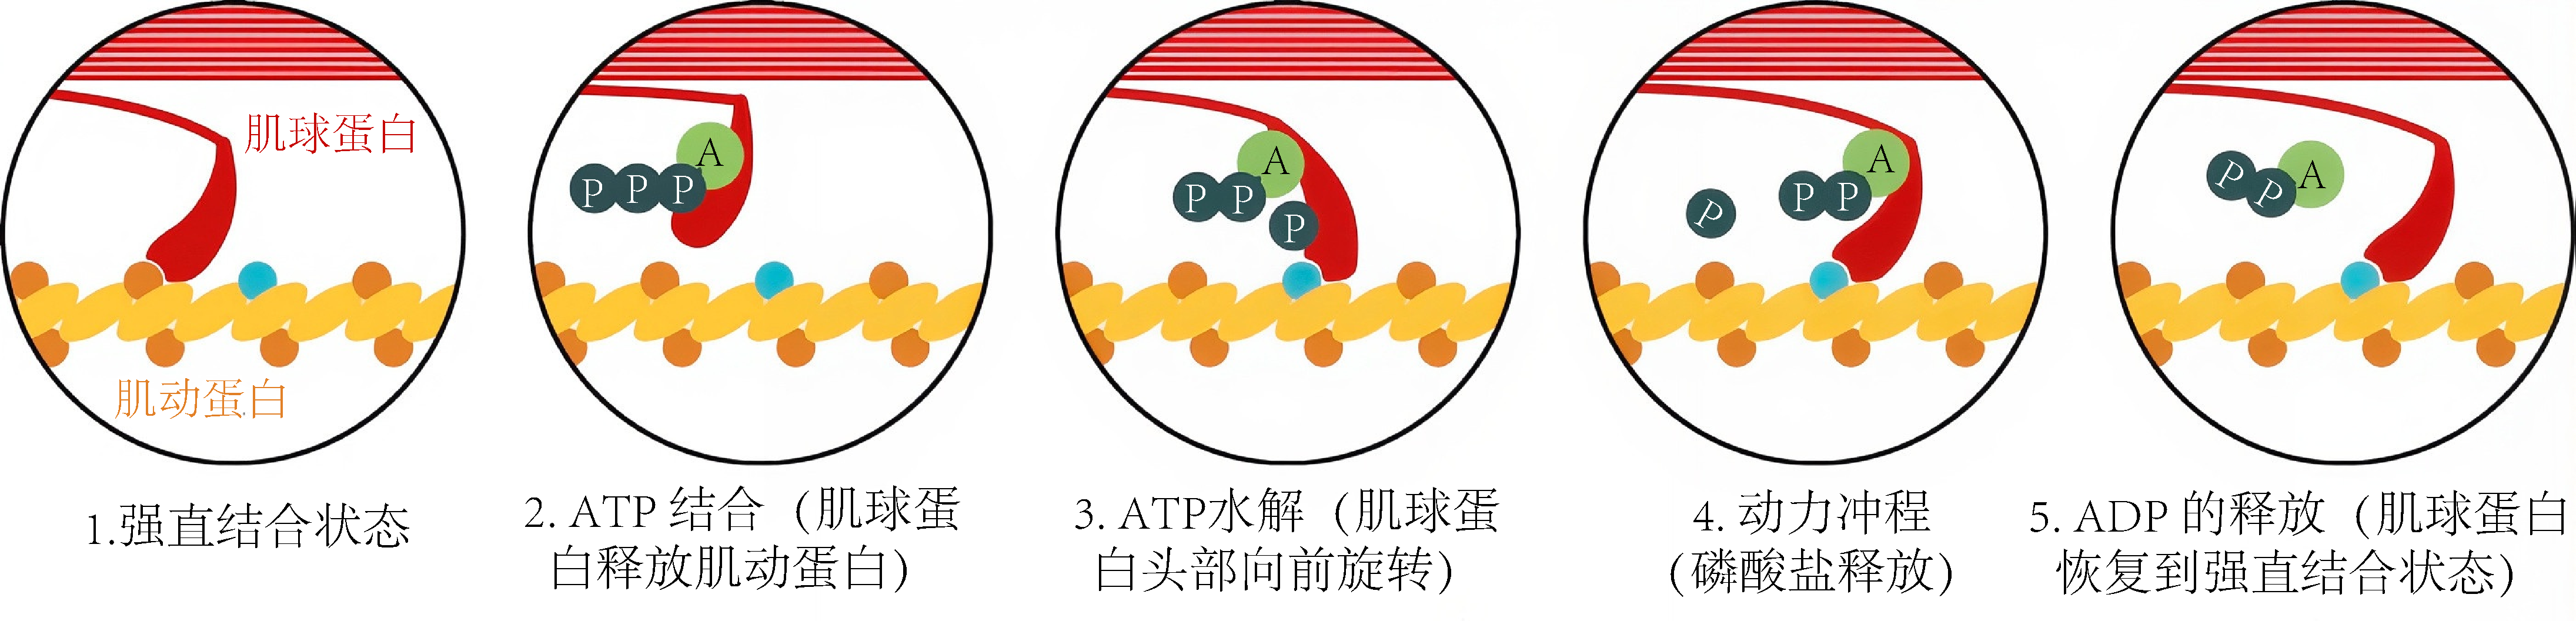
\includegraphics[width=1.0\linewidth]{chap4/4_3}
	\caption{横桥循环描述了肌动蛋白和肌球蛋白相互作用产生力量和运动的过程。
		A 代表腺苷;P 代表磷酸。 \label{fig:4_3}}
\end{figure}

肌球蛋白分子分为 3 个区域,分别称为头部、颈部和尾部。
肌球蛋白头部的独特结构使其能够牢固地结合到肌动蛋白丝上的特定位置(图~\ref{fig:4_3}~第一帧)。
当肌肉需要产生力量时,肌球蛋白头部会接收一种名为三磷酸腺苷 (ATP) 的“燃料”分子。
这刺激肌球蛋白头部从肌动蛋白上分离,向前旋转,并附着到肌动蛋白上的下一个结合位点(图~\ref{fig:4_3}~第二帧和第三帧)。
接下来,肌球蛋白头部围绕颈部区域旋转,这一运动被称为动力冲程 (power stroke),产生几皮牛顿的力,并使肌动蛋白丝彼此滑动约 10 纳米。


当然,不消耗能量就不可能完成机械功。
能量来自于一个化学反应,该反应将一个磷酸离子从三磷酸腺苷中分离出来(图~\ref{fig:4_3}~中的图4),留下二磷酸腺苷(ADP)。
最终,二磷酸腺苷被释放,肌球蛋白恢复到其原始状态,但现在已从其原始位置移位。
当肌球蛋白以这种方式循环时,细丝被拉向肌节中部,从而在化学能转化为机械能的过程中产生张力。


虽然这种机制听起来可能很复杂,但它却是一个优雅而经济的解决方案,解决了如何在分子层面上以可预测的方向产生力的问题。
就像汽车发动机一样,我们的肌肉将化学能转化为机械能,但噪音更小,产生的有毒废气也更少。



\section{肌节结构}

再往上一层,我们来看看肌节。
肌节大致呈圆柱形,长度根据肌肉长度在 1 微米到 5 微米之间变化。
肌节由许多相互交织的“粗”肌丝和“细”肌丝组成,随着肌节长度的变化,这些肌丝会相互滑动。


数百条肌球蛋白尾部捆绑在一起,形成每根粗肌丝,形成棒状结构,肌球蛋白头部以规则的间隔向外放射状延伸(图~\ref{fig:4_4})。
与粗肌丝平行的是细肌丝,它们由 3 种蛋白质组成:
肌动蛋白、原肌球蛋白和肌钙蛋白。
我们已经描述了肌动蛋白,它为肌球蛋白头部提供结合位点。
这些结合位点沿着细肌丝以规则的间隔分布。
原肌球蛋白和肌钙蛋白仅在肌肉被神经系统激活且存在钙离子时才会暴露这些结合位点,从而帮助调节力量的产生。
另一种值得关注的蛋白质(肌联蛋白),将每根粗肌丝附着在肌节的末端(我们称之为 Z 线或 Z 盘)。
正如我们稍后将看到的,肌联蛋白在被动力的产生中起着重要作用,这是一个独立于横桥循环的过程,也是赫胥黎最初的模型所忽略的现象。

\begin{figure}[!htb]
	\centering
	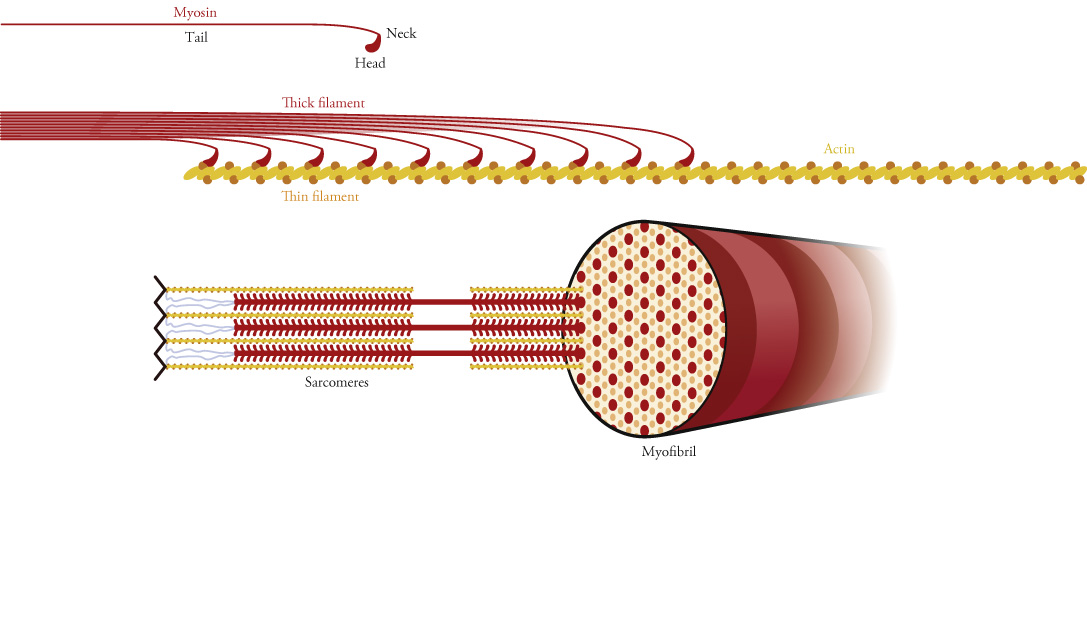
\includegraphics[width=1.0\linewidth]{chap4/4_4}
	\caption{肌球蛋白示意图(顶部)、粗丝和细丝的相互作用示意图(中间)以及肌原纤维横截面,显示粗丝和细丝以高度有序的三维模式排列(底部)。 \label{fig:4_4}}
\end{figure}

肌节在骨骼肌内以规则的模式串联和平行排列,在显微镜下观察骨骼肌组织时,会形成条纹,即明暗交替的带状结构。
您可以在图~\ref{fig:4_5}~中看到这些带状结构,它们分别被称为 I 带、A 带、Z 盘和 M 盘。
严格来说,Z 盘和 M 盘确实是圆盘,但它们通常被称为 Z 线和 M 线,因为它们在二维空间中看起来是这样的。
A 带仅出现在含有肌球蛋白的区域,而 I 带则出现在其他区域。细肌动蛋白丝的一端锚定在 Z 盘上。
粗肌球蛋白丝的一端附着在 M 盘的结构上,另一端通过肌联蛋白分子固定在 Z 盘上。
骨骼肌有时被称为“横纹肌”,与“平滑肌”相对,例如控制血管口径的肌肉,它们没有组织成肌节,也没有呈现条纹图案。

\begin{figure}[!htb]
	\centering
	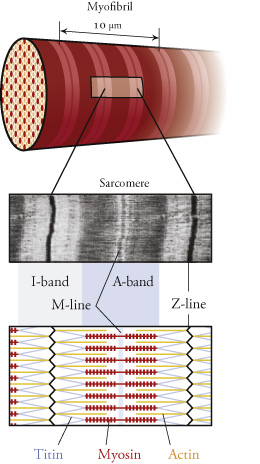
\includegraphics[width=0.5\linewidth]{chap4/4_5}
	\caption{肌原纤维示意图(上)展示了其高度组织化的微观结构。
		肌肉显微镜图像(中)和肌节示意图(下)分别标记了I带、A带、M线和Z线。
		肌节的末端由Z线定义。 \label{fig:4_5}}
\end{figure}


\section{力-长度关系}

肌节所能产生的最大力量会随着其长度的变化而变化。
长度和张力之间的关系可以用滑动丝理论来解释,该理论由两个研究小组于 1954 年独立提出。
Andrew Huxley 和 Rolf Niedergerke(在单根肌纤维中)以及 Hugh Huxley 和 Jean Hanson(在分离的肌原纤维中)证明,在主动肌肉收缩过程中,肌小节带不会变窄,这推翻了粗肌丝缩短的流行理论。
他们给出的解释是,随着肌节长度的变化,粗肌丝和细肌丝会相互滑动。
因此,肌节的长度会影响肌动蛋白和肌球蛋白之间“重叠”的量,或者说靠近细肌丝上结合位点的肌球蛋白头部的数量。
随着肌球蛋白头部和肌动蛋白结合位点之间横桥数量的增加,激活的肌节内的张力也会增加。


如图~\ref{fig:4_6}~所示,激活的肌肉中横桥循环所能产生的力随肌节长度而变化。
该主动力-长度曲线通常被描述为具有三个区域:
上升区,其中力随肌节长度的增加而增加;
平台区,其中力保持在最大值;
下降区,其中力随肌节长度的增加而减小。
平台区涵盖一系列肌节长度,称为“最佳”范围,其中肌球蛋白头部和肌动蛋白结合位点之间的相互作用数量达到最大值。
最佳肌节长度因脊椎动物而异,但通常在 2.2 至 2.7 μm 之间,在人类骨骼肌中约为 2.7 μm。
当肌节长度超过最佳范围时,肌动蛋白和肌球蛋白的重叠量会减少,横桥循环所能产生的力量也会减少。
当肌节长度略短于最佳长度时,源自肌节两端的细肌丝开始在肌节中部重叠并相互干扰,导致所谓的“浅上升区”的力量减弱。
当肌节长度更短时(在“陡峭上升区”),粗肌丝会与Z盘碰撞并变形,产生阻碍横桥循环作用的力量。
由于肌肉由串联和并联排列的肌节组成,我们可以观察到肌肉主动收缩过程中力量与长度之间的类似关系。

\begin{figure}[!htb]
	\centering
	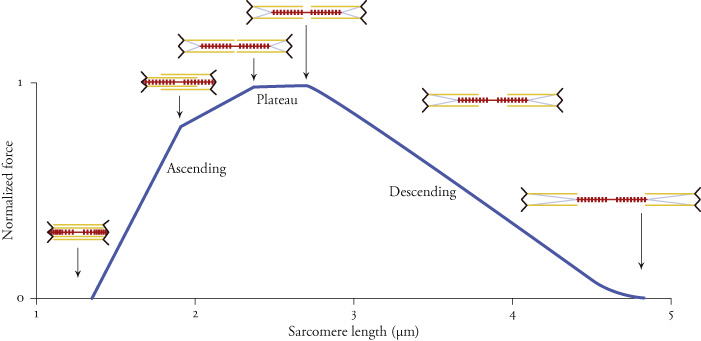
\includegraphics[width=0.5\linewidth]{chap4/4_6}
	\caption{肌节产生的主动力与其长度有关。粗肌丝和细肌丝相互滑过时,力会发生变化。
		在肌节的上升支,力随长度增加而增大,达到平台期;
		在肌节的下降支,力随长度增加而减小。
		当横桥数量达到最大时,力的产生达到峰值\cite{gordon1966variation}。 \label{fig:4_6}}
\end{figure}




